\selectlanguage{english}%

\chapter{Sistemas Fuzzy} \label{capFundFuzzy}
A lógica fuzzy, ou difusa, foi introduzida originalmente por Lofti A. Zadeh, em seu artigo "Fuzzy sets and systems" \cite{zadeh}. Sua teoria diverge da lógica booleana convencional no tratamento da pertinência das variáveis, podendo assumir qualquer valor entre todos os possíveis de um intervalo. Essa abordagem é mais eficaz na descrição de alguns sistemas reais, uma vez que é praticamente eliminar incertezas nos modelos que os representam. Este capítulo apresenta os fundamentos desse paradigma bem como sua aplicação na modelagem, proposta por Takagi e Sugeno \cite{takagiSugeno}.

\section{Conjuntos Fuzzy}
De acordo com a teoria de conjuntos clássica, um elemento $x$ qualquer, pode pertencer ou não à um conjunto universo de discurso $U$, $x \in U$. Ou seja, para qualquer conjunto determinado, pode-se estar completamento dentro ou completamente fora dele. Como exemplo, $f_u(x)$ a função de pertinência de $x$ ao conjunto $U$, tem-se:

\begin{align}
	f_u(x) : U \rightarrow \{0,1\}
	&& f_u(x) =
	\begin{cases*}
		1 & se e somente se $x \in U$ \\
		0 & caso contrário
	\end{cases*}
	\label{eqFPertinencia}
\end{align}

Essa definição binária se encaixa bem em problemas restritos, cujo caráter dos sistemas reflita essa separação clara de estados, por exemplo a paridade ou não de uma da soma dos bits de uma mensagem binária. Este valor ou é "completamente" ímpar ou par. No entanto, grande parte dos sistemas estudados nas teorias de controle trabalha com grandezas que não possuem limites tão claros assim, como exemplo a sensação térmica. Apesar de a temperatura ser matematicamente bem definida, existem descrições como "frio" e "quente" que não podem ser representadas com este conjunto binário, uma vez que são conceitos vagos e imprecisos.

A abordagem fuzzy aparece como uma alternativa muito capaz de tratar estes casos. Conjuntos fuzzy são caracterizados por uma função de pertinência fuzzy, que relaciona cada elemento do universo discurso à sua conformidade no conjunto de forma contínua, podendo abranger todos os valores no intervalo de pertinência.

\subsection{Variáveis Linguísticas}
As variáveis linguísticas são objetos que constituem os conjuntos nebulosos. Tratam-se de traduções das variáveis reais na forma de valores linguísticos, não números. Assim, prosseguindo o exemplo anterior, a temperatura seria a variável linguística e "quente", "frio", "muito quente" e "muito frio" seus valores linguísticos. Estes últimos são os conjuntos difusos e possuem, cada um deles, uma função de pertinência mapeando a adequação de uma determinada temperatura a eles.

\section{Funções de Pertinência}
\label{secFncPert}
O conceito chave de toda a abordagem fuzzy são as funções de pertinência. Em exemplo, dados os conjuntos fuzzy $U_1$, $U_2$ e $U_3$, cada qual possui sua função de pertinência $f_1(x)$, $f_2(x)$ e $f_3(x)$, para todo elemento pertencente ao universo de discurso.

\begin{align}
	f_i(x) : i \rightarrow [0,1]
	\label{eqFuncPertFuzzy}
\end{align}
Onde $f_i(x)=0$ implica que o elemento $x$ é "completamente não" $U_i$ e $f_i(x)=1$ indica que $x$ é "completamente" $U_i$.

Apesar de traduzir operar sobre grandezas linguísticas, é importante notar que normalmente os elementos são variáveis numéricas, portanto as funções de pertinência precisam ser bem definidas no intervalo do conjunto. Os formatos mais comuns para elas são apresentados na \hyperref[figPert]{Figura \ref{figPert}} a seguir:

\begin{figure}[H]
	\centering
\begin{tabular}{ccc}
	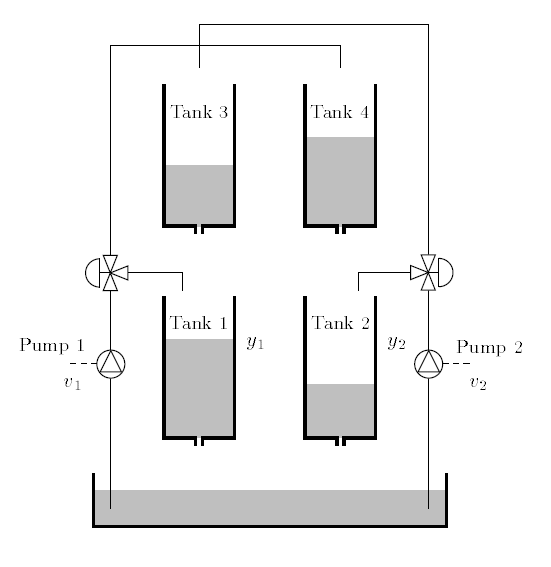
\includegraphics[width=0.3\textwidth,keepaspectratio]{img/4tank.png} &
	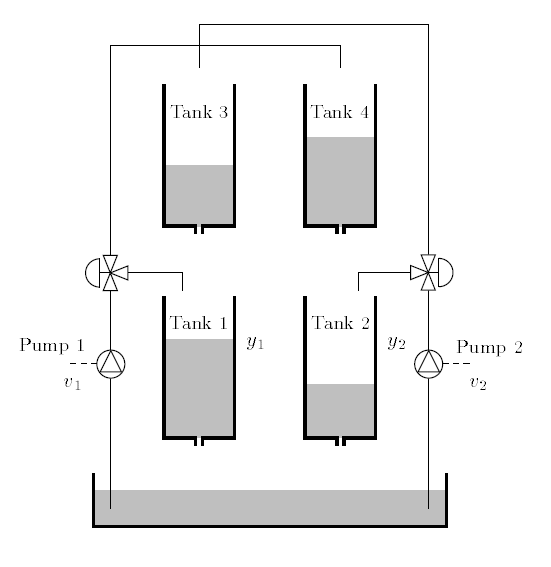
\includegraphics[width=0.3\textwidth,keepaspectratio]{img/4tank.png} &
	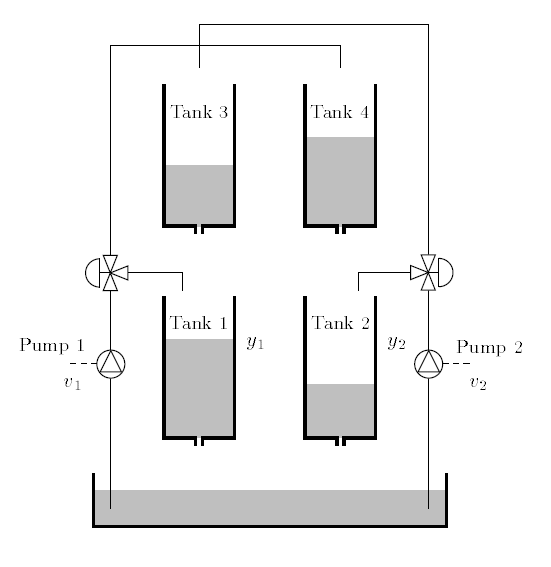
\includegraphics[width=0.3\textwidth,keepaspectratio]{img/4tank.png} \\
	(a) Primeira &
	(b) Segunda &
	(c) Terceira \\
	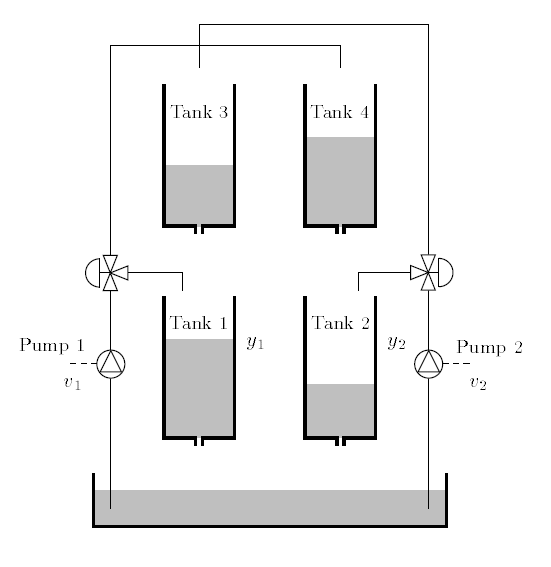
\includegraphics[width=0.3\textwidth,keepaspectratio]{img/4tank.png} &
	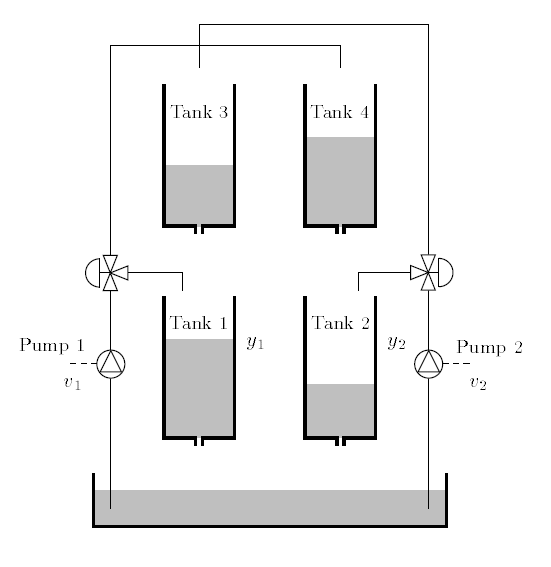
\includegraphics[width=0.3\textwidth,keepaspectratio]{img/4tank.png} &
	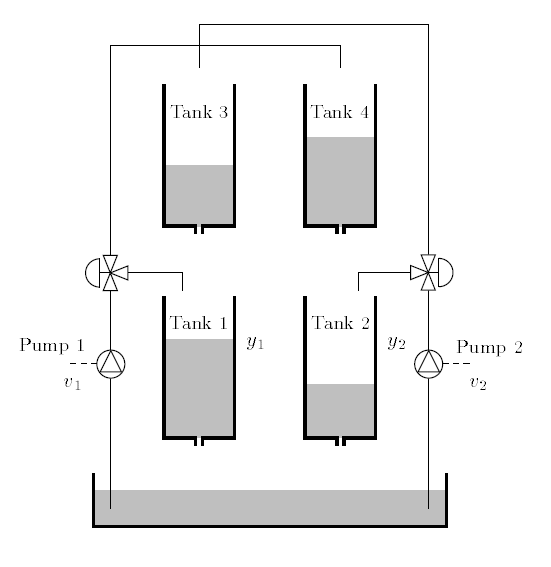
\includegraphics[width=0.3\textwidth,keepaspectratio]{img/4tank.png} \\
	(d) Quarta &
	(e) Quinta &
	(f) Sexta
\end{tabular}
	\caption{\label{figPert}Funcões de Pertinência.}
\end{figure}

Voltando ao exemplo temperatura, segue-se abaixo o procedimento para definição:
\begin{itemize}
	\item \textbf{Definir os conjuntos fuzzy:} \{"muito frio"\}, \{"frio"\}, \{"quente"\}, \{"muito quente"\}
	\item \textbf{Definir os limites de cada conjunto:} $[-10ºC,5ºC]$,$ [5ºC,15ºC]$, $[15ºC,30ºC]$, $[30ºC,45ºC]$ 
	\item \textbf{Definir as funções de pertinência:} Funções triangulares, com picos nos centros dos intervalos e zeros fora deles.
\end{itemize}

Os resultados do exemplo são apresentados na \jhhref{figPertEx}{Figura} a seguir:
\begin{figure}[H]
	\centering
	\begin{tabular}{cc}
		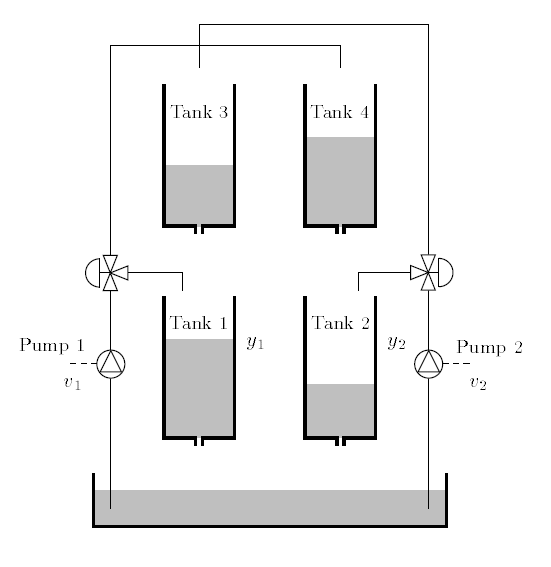
\includegraphics[width=0.3\textwidth,keepaspectratio]{img/4tank.png} &
		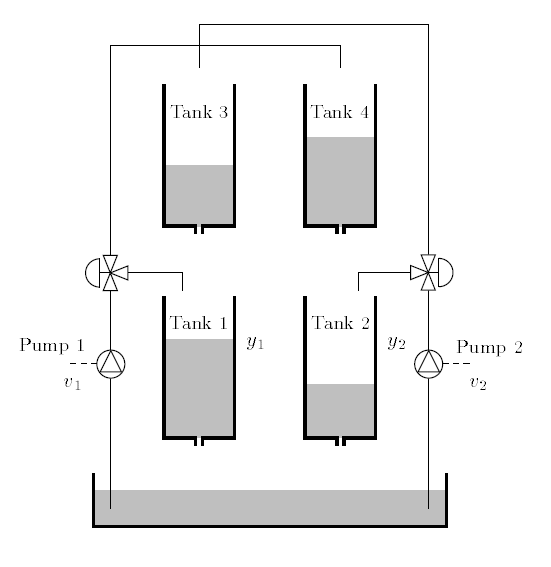
\includegraphics[width=0.3\textwidth,keepaspectratio]{img/4tank.png} \\
		(a) Primeira &
		(b) Terceira \\
		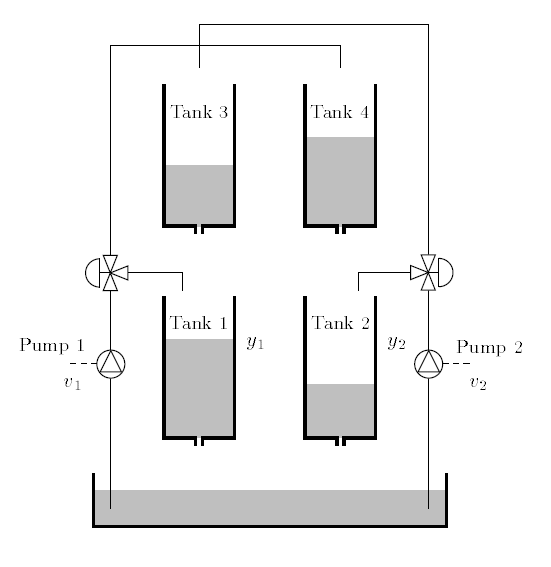
\includegraphics[width=0.3\textwidth,keepaspectratio]{img/4tank.png} &
		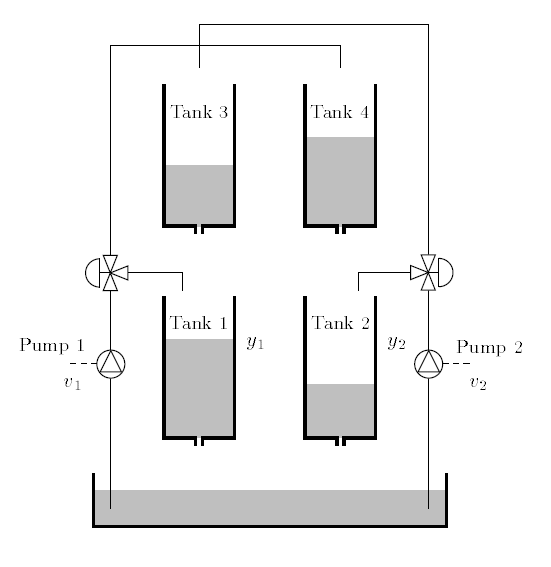
\includegraphics[width=0.3\textwidth,keepaspectratio]{img/4tank.png} \\
		(c) Quarta &
		(d) Sexta
	\end{tabular}
	\caption{\label{figPertEx} Funções de Pertinência.}
\end{figure}	

\begin{table}[!ht]
	\caption{Tabela de Exemplos}
	\label{tabPertEx}
	\small
	\centering
	\scalebox{1}{
		\begin{tabular}{|c|c|c|c|c|}
			\hline
			Temperatura & Muito Frio & Frio & Quente & Muito Quente \\
			\hline
			0 & 0 & 0 & 0 & 0 \\
			\hline
			0 & 0 & 0 & 0 & 0 \\
			\hline
			0 & 0 & 0 & 0 & 0 \\
			\hline
			0 & 0 & 0 & 0 & 0 \\
			\hline
			0 & 0 & 0 & 0 & 0 \\
			\hline
			0 & 0 & 0 & 0 & 0 \\
			\hline
			0 & 0 & 0 & 0 & 0 \\
			\hline
			0 & 0 & 0 & 0 & 0 \\
			\hline
		\end{tabular}
	}
\end{table}

É importante notar que a soma final dos valores de todas as pertinências de um elemento precisa ser 1, para que haja coerência entre o modelo dos conjuntos e o real.

\section{Aplicação}
A aplicação da 
lógica fuzzy na teoria de controle se dá através da utilização de regras que definem o modelo final baseando-se no grau de pertinência do estado do sistema a cada um dos conjuntos difusos. 

De maneira similar à tradicional, a lógica fuzzy baseia-se no paradigma de implicações, ou \textit{modus ponens}. De acordo com esta linha de raciocínio, definem afirmações premissas que quando verdadeiras determinam a autenticidade de afirmações conclusões. Por exemplo:

\begin{align} \label{eqRegrasEx}
\begin{cases}
	\text{(1) Se está  chovendo então é perigoso dirigir}\\
	\text{(2) Está chovendo }\\
	\text{(3) É perigoso dirigir}
\end{cases}		
\end{align}

No \jhhref{eqRegrasEx}{exemplo} a afirmação (1) é chamada de regra de implicação, ou regra Se-Então, e é ela quem rege o comportamento da conclusão (3) de acordo com a premissa (2).

\subsection{Regras Se-Então}
Como visto no \jhhref{eqRegrasEx}{exemplo} as regras Se-Então são as premissas que definem os resultados das afirmações 
Regras Se-Então e o raciocínio fuzzy formam o cerne da vasta gama de sistemas fuzzy encontrados
na literatura (Jang et al., 1997). Uma regra Se-Então (também conhecida como regra
fuzzy, implicação fuzzy ou proposição condicional fuzzy) tem a seguinte forma
R :
Se x é A
Então y é B
(2.4)
onde R identifica a regra; A e B são variáveis lingüísticas; x, y são elementos dos universos
de discurso X, Y , respectivamente. Normalmente, denomina-se a proposição x é A como
antecedente, enquanto y é B é chamado conseqüente (ou conclusão); x é chamada de variável
premissa.
Na concepção tradicional, ativa-se (dispara-se) uma regra Se-Então somente quando a
variável premissa x é exatamente igual ao antecedente. Neste caso, a inferência produzida
será: y é exatamente igual ao conseqüente

	\textbf{Regra i:}
	\begin{align}
		&\textbf{SE:} \text{ $v_1(t)$ é $M_{i1}$ e $v_2(t)$ é $M_{i2}$ e ... e $v_n(t)$ e $M_{in}$,} \\
		&\textbf{ENTÃO}: \ \ \begin{cases}
			\dot{x}(t) = A_ix(t) + B_iu(t),\\
			y(t) = C_ix(t)
		\end{cases}
	\label{eqRegraIGeral}
	\end{align}
	
	\textbf{Regra i:}
	\begin{align}
		\textbf{SE:}  \hspace{1cm} &\text{ $h_1(t)$ é $P_{1,i}$ e $h_2(t)$ é $P_{2,i}$,} \\
		\textbf{ENTÃO:} \hspace{1cm} & \dot{h}(t) =  A_i \Delta h_i(t) +  B_i \Delta u_i(t)
	\end{align}
	
	Cada regra definida implica um sistema linear diferente, que melhor representa a dinâmica da planta em cada região. Essas linearizações são baseadas nas variáveis de desvio, assim, para cada regra $i$, temos:
	\begin{align}
		\Delta h_i(t) =
		\begin{bmatrix}
			h_1(t) - \bar{h_{1i}} \\
			h_2(t) - \bar{h_{2i}} \\
			h_3(t) - \bar{h_{3i}} \\
			h_4(t) - \bar{h_{4i}}
		\end{bmatrix} 
		&&
		\Delta u_i(t) = 
		\begin{bmatrix}
			u_1(t) - \bar{u_{1i}} \\
			u_2(t) - \bar{u_{12}}
		\end{bmatrix}
	\end{align}	

\section{Inferência}
Sistemas de inferência são ferramentas computacionais utilizadas nas mais diversas áreas
da Engenharia e agregam os conceitos de conjuntos fuzzy, variáveis lingüísticas e raciocínio
aproximado, processando dados por meio de mecanismo de inferência. A estrutura básica de
um sistema de inferência é mostrada na Figura 2.4.
Sistemas de inferência normalmente, embora não seja obrigatório, recebem como entrada
valores precisos5. Isto ocorre pois, na prática, os dados de entrada são obtidos por meio de
medições ou observações. É necessário portanto a etapa chamada fuzzificação, que transforma
entradas precisas em conjuntos fuzzy.
Após a interpretação das entradas pelo mecanismo de inferência, etapa identificada como
inferência na Figura 2.4, é necessário fornecer uma informação precisa. No caso de um sistema
5Também chamadas entradas “crisp”
2. Fundamentos Fuzzy 11
PSfrag replacemen
Entradas
Precisas Precisas
Saídas
Conjuntos Conjuntos ou Funções
Fuzzy Fuzzy
Fuzzificação
Regras
Defuzzificação
Inferência
Figura 2.4: Diagrama esquemático do sistema de inferência.
No estágio de inferência ocorrem as operações com conjuntos fuzzy ao longo de regras Se-
Então para processar, por meio de um mecanismo de inferência, as informações da entrada e
produzir uma conclusão.
A inferência pode ser resumida em quatro etapas (Jang et al., 1997). Em uma primeira
instância, são avaliados os graus de compatibilidade das variáveis premissas com seus respectivos
antecedentes nas regras Se-Então. Considerando o caso da regra (2.4), isto significa
atribuir uma pertinência da variável x no conjunto A.
Em seguida, é necessário determinar a força (grau) de ativação de uma regra. O grau de
ativação da regra é dado pela combinação dos graus de compatibilidade das variáveis premissas
com seus antecedentes. Na regra (2.5) cada antecedente (x é A), (z é C), produz um grau
de compatibilidade, fA(x), fC(z). De acordo com os conectivos lógicos presente na premissa
da regra e do tipo de norma adotada, obtém-se um grau de ativação para a regra R, veja na
Figura 2.5 denotado por . Caso em (2.5), por exemplo, fosse utilizado o conectivo “ou” o
resultado produzido seria diferente.
Com base no grau de ativação determina-se o conseqüente produzido por uma determinada
regra, chamado conseqüente induzido. Considere novamente a regra (2.5). Se o grau de
ativação desta regra é 1, significa que o conseqüente produzido é o próprio B. Ademais, de
acordo com o grau de ativação, o conseqüente terá um grau de pertinência em B, i.e, y é B.
Não raro um sistema de inferência possui mais de uma regra. Cada regra produz um
conseqüente e o resultado global da etapa inferência dependerá da combinação desses conseqüentes.
Esta etapa é chamada de agregação, a qual tem por resultado um conjunto fuzzy
(função de pertinência) ou uma função.

\section{Modelo Fuzzy Takagi-Sugeno}
\label{secTakSug}

	\begin{equation}
	\begin{aligned}
		w_{1}(t) = M_1(h_1(t)) * N_1(h_2(t)) \\
		w_{2}(t) = M_1(h_1(t)) * N_2(h_2(t)) \\
		w_{3}(t) = M_2(h_1(t)) * N_1(h_2(t)) \\
		w_{4}(t) = M_2(h_1(t)) * N_2(h_2(t))
	\end{aligned}
	\end{equation}
	
	\begin{align}
		\dot{h}(t) = \frac{\sum_{i=1}^{4}  w_i(h(t))(A_i \Delta h_i(t) +  B_i \Delta u_i(t))}{\sum_{i=1}^{4} w_i(h)}
	\end{align}

Na concepção fuzzy, a regra Se-Então é disparada quando houver um grau de similaridade
não nulo entre a variável premissa e o antecedente. Como resultado, infere-se uma conclusão
que mantenha algum grau de similaridade com o conseqüente da regra. Nota-se, mais uma
vez, que os conceitos tradicionais estão embutidos na teoria fuzzy. Se a variável premissa x
possui total similaridade com o antecedente A então a conclusão será que y é o próprio B.
Uma regra fuzzy pode possuir mais de um antecedente. Um exemplo simples é dado a
seguir:
R :
Se x é A e z é C
Então y é B
(2.5)
Neste caso, a maneira de inferir uma conclusão é bem mais elaborada. A conclusão depende
tanto da similaridade de x em A, quanto da similaridade de z em C. Além disso, depende da
relação entre ambos antecedentes, bem como da relação deles com o conseqüente.
Por exemplo, considere um veículo trafegando em uma estrada. Uma regra com múltiplos
antecedentes para inferir sobre a velocidade adequada do carro pode ser: “se a curva é fechada
ou a pista está molhada, então dirija em baixa velocidade”.
No caso de pista seca, quanto mais fechada for a curva, menor deve ser a velocidade.
Em outras palavras, quanto maior for a pertinência da variável “curva” no conjunto fuzzy
“fechada”, maior deverá ser a pertinência da “velocidade” no conjunto “baixa”.
Se o carro viaja pela mesma curva porém com pista molhada, por questão de segurança,
a velocidade deverá ser ainda menor. Neste caso a pertinência da “velocidade” no conjunto
“baixa” será afetada também pelo valor lingüístico da variável “pista”.
Existem diversas configurações que definem como os antecedentes interagem entre si e
com o conseqüente da regra para produzir uma conclusão. Tais configurações são chamadas
mecanismos de inferência e podem ser vistos com maiores

\indent A Teoria Fuzzy tem seu princípio cunhado por \cite{zadeh65}. Os trabalhos seguintes, como o \cite{takagi_sugeno} abordaram sua utilização para a modelagem de sistemas complexos por meio de aproximações, utilizando uma teoria de conjuntos diferente da convencional.

\subsection{Conjuntos Fuzzy}
\indent A teoria de conjuntos convencional utiliza lógica booleana para definir os valores lógicos das funções de pertinências dos conjuntos. Assim, dado $X$ o universo de discurso de um determinado conjunto $C$, um elemento genérico $x$ tem sua função de pertinência ao conjunto $C$ dado por:

\begin{align*}
f_{C}(x)&:X \rightarrow \{0,1\} \quad \\
f_{C}(x)&= 
\begin{cases}
1 \text{ se e somente se x} \in C \\
0 \text{ se e somente se x} \notin C\\
\end{cases}
\end{align*}

Existem, no entanto, situações em que a definição dos conjuntos de seus limites se tornam muito subjetivos. Nestas situações, a utilização da lógica difusa apresenta vantagens para a modelagem de sistemas. 

Considere-se como exemplo a temperatura de uma sala. Pode-se definir dois conjuntos de estados \{quente,frio\}. No entanto, torna-se um pouco confuso e arbitrário decidir em qual destes conjuntos um estado específico se encaixa. Utilizando funções de pertinências não binárias, observa-se o \textbf{quanto} determinada temperatura se encaixa em cada um dos conjuntos. Funções de pertinências fuzzy são definidas da forma:

\begin{align*}
f_{C}(x)&:X \rightarrow [0,1]
\end{align*}

\subsection{Funções De Pertinência}
Existem várias normas e regras disponíveis para funções de pertinência. Este trabalho considera a norma triangular. Seguindo o exemplo dado, dada uma temperatura $x$ verifica-se o quão pertencente aos conjuntos \textit{quente} e \textit{fria} ela é utilizando a função do gráfico a seguir:

\begin{figure}[H]
	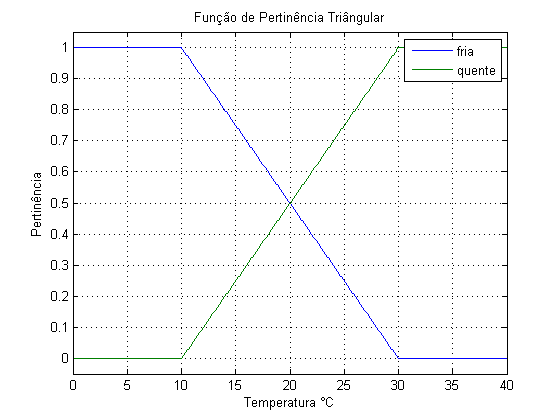
\includegraphics[width=0.5\textwidth]{img/pertinencia.png}
	\caption{Diagrama esquemático do sistema de quatro tanques e planta didática.}
	\label{figPertinencia}
\end{figure}

Nota-se que se escolhem limites para os conjuntos: toda temperatura abaixo de 10 é fria; toda temperatura acima de 30 é quente. As demais, pertencem mais ou menos à cada um dos conjuntos.

Em lógica Fuzzy, as variáveis definidas de forma subjetiva, com expressões para limites são chamadas variáveis linguísticas.




\selectlanguage{brazil}%

